\documentclass[11pt,oneside,a4paper]{article}
\usepackage{graphicx}
\usepackage{booktabs}
\usepackage{caption}
\usepackage{subcaption}
\usepackage{amsmath}
\usepackage{amsfonts}
\usepackage{amssymb}
\usepackage{lscape}
\usepackage{psfrag}
\usepackage[usenames]{color}
\usepackage{bbm}
\usepackage[update]{epstopdf}
\usepackage[bookmarks,pdfstartview=FitH,a4paper,pdfborder={0 0 0}]{hyperref}
\usepackage{verbatim}
\usepackage{listings}
\usepackage{textcomp}
\usepackage{fancyhdr}
\usepackage{multirow}
\usepackage{tikz}
\usepackage{lipsum}

\usepackage{xcolor}
\usepackage[margin=1in]{geometry}
\newcommand{\hint}[1]{{\color{blue} \em #1}}
\newenvironment{tty}
{\small\begin{alltt}}
{\end{alltt}}
\lstset{breaklines=true} 
\lstset{basicstyle=\scriptsize\ttfamily}
\makeatletter
\def\cleardoublepage{\clearpage\if@twoside \ifodd\c@page\else%
\hbox{}%
\thispagestyle{empty}%
\clearpage%
\if@twocolumn\hbox{}\clearpage\fi\fi\fi}
\makeatother

\sloppy
% \widowpenalty=10000
% \clubpenalty=10000

\title{
    \vspace*{0.0mm}
    \LARGE\bf\sf Advanced Topics in \\Communication Networks (Fall 2019)
    \vspace*{10.0mm} \\
    \Large\bf\sf Group Project Report \vspace*{30.0mm}\\
    %
    \Huge\bf\sf NetChain: Scale-Free Sub-RTT Coordination
    %
    \vspace*{30.0mm} \\
    \normalsize
    %
    \sf Authors:\\[5pt]
    \sf Haoyu Zhu \\ [5pt]
    \sf Francisco Dumont \vspace*{5mm}\\
    %
    \sf  Advisor: Thomas Holterbach \vspace*{5mm}\\
    %
    \sf  Supervisor:  Prof. Dr. Laurent Vanbever \vspace*{20.0mm}\\
    %
    \sf Submitted: Dec 16, 2019\\ [5pt]
    \sf \pageref{lastpage} Pages
}
\date{}

\begin{document}

\begin{figure}
    
\includegraphics[width=\textwidth]{figures/eth-nsg-header}
\end{figure}

\maketitle
\thispagestyle{empty}
\raggedbottom
\clearpage

\pagenumbering{roman}

\begin{abstract}
    This report focus on the p4 implementation of the paper "NetChain: Scale-Free Sub-RTT Coordination"\cite{211261} published in the 15th USENIX Symposium. For the implementation of this paper a virtual machine with linux was used, which had all necessary python, p4, c and minimet tools. NetChain is an in-network solution for coordination services. By coordinating within the network, the Sub-RTT system can reduce query latency, maintain higher throughput, can be scaled easily and provide consistency in the presence of failures.
    The implementation  will be explained in three different levels: Host, Controller and Switch Data Plane. The host was implement in c, most of the controller in python and the data plane in p4. 
    As the implementation is done in a virtual machine, the evaluation aspects are limited. Despite the limitations, the evaluation focus on the correct functionality of the different operations, protocols and the time interval that the throughput is affected by a failure and its recovery.

\end{abstract}

\clearpage
\setcounter{tocdepth}{3}
\tableofcontents
\clearpage
\pagenumbering{arabic}

\section{Introduction}

Networks are about to experience mayor changes with the introduction of programmable switches. This new tool open the possibility to solve current challenges in a more efficient, fault-tolerant, consistent and innovative way. One of those challenges is the how to increase the performance of coordination systems, which up to this day use a server-based solution. Programmable Switches open the possibility to use an alternative approaches by using the switches in the network as data storage. This take advantage of how fast switches can process packets in comparison with a traditional solution.

\subsection{Goal}
The goal of this implementation is to write the required code to have a working NetChain system in a virtual machine. The implementation tries to stay in line with the paper as much as possible, but some implementation decisions had to be made in order fulfill some aspects that weren't explicitly stated in the paper. 

\subsection{Paper summary}

To start, two  mayor ideas of protocols have to be recognised: Steady state and reconfiguration protocol. The first one deals with read and write operations of data, which is mainly performed in the data plane. The second protocol will use the network control plane for reconfiguration operations like joining (insert a new key), leaving (delete a key), failure behaviour behaviour and scalability. 

The First building block of the NetChain system is the concept of 'Chain Replication', which can be described as a virtual nodes organized in a chain structure with a head and a tail. This chain of virtual nodes is placed along different real switches and the key-value information is replicated in each one of them. The next building block in the system are the virtual nodes themselves. These are an abstraction used to evenly spread the data storage between the real switches. The virtual nodes with the help of consistent hashing are mapped to a hash ring, meaning that each node is responsible for a certain amount of hashing values. A mapping of virtual nodes and real switches has to be made.

NetChain uses an additional packet structure implemented in the UDP payload, which is shown in figure\ref{fig:netchainpkt}. The packet is organized in the following order: First, a count of how many switches the packet still has to go through, followed by the IP addresses of those switches. Then the operation to be performed. Third, a sequence number for the key. And Finally the key  and its particular value. The IP addresses chain only shows the ordered path of switches the packet has to visit, but the routing between two of them is left to the IP protocol. This means, in the IPv4 protocol the destination address is updated depending on the next switch in the chain. Thus, once the destination is reached, the counter is reduced by one and the next IP address in the chain is updated to the IPv4 protocol. The operations described in the paper are insert, delete, write and read. Inserting a key requires the controller to assign a register index to that key in each switch and keep track of it in all the virtual nodes it is assigned to. The delete action also needs the controller to act so that it can free the memory register in the switches and erase the key from the virtual nodes. On the other hand , the write and read operation doesn't need any controller involvement. While write operations will travel trough each one of the switches in the chain starting from the head, the reading will only go to the tail to, get the value and sent it back to the host.

\begin{figure}[h]
    \centering
    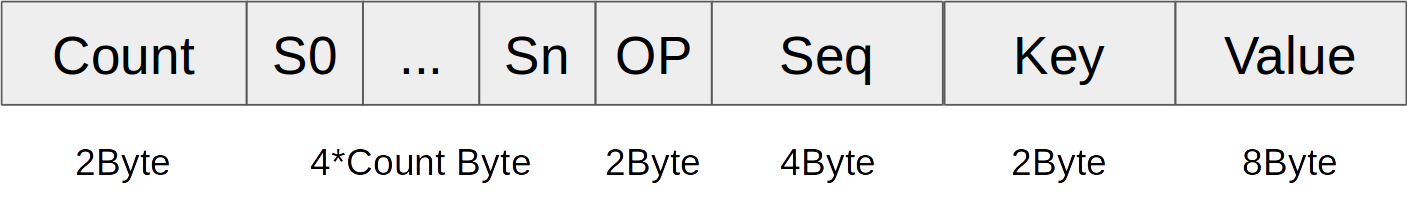
\includegraphics[width=0.8\textwidth]{figures/NetChain-packet.png}
    \caption{NetChain packet structure used in our project}
    \label{fig:netchainpkt}
\end{figure}

The next component in the packet structure is the sequence number. This helps to keep the saved values of each key updated in the correct order. Once a packet arrives at the designated switch, the sequence number is compared. If it is lower than the one saved in the switch the packet will be dropped, otherwise the value is updated and the packet forwarded to the next destination.

In the case a certain switch fails, two processes can be described. This first is fast-failover, here the controller quickly reconfigures the neighbor switches of the failed one in a way to bypass it and continue to the next IP address in the chain or send it back to the host if the failed switch was in the tail. The second procedure is failure-recovery. The goal of this procedure is to replace the failed switch with another. In this regard the controller has to perform two mayor things. To start it has to reconfigure the mapping of virtual nodes and real switches. Second, insert the needed keys into the new mapped switches and once this is done the fast failover state can be lifted, so that the packets can travel through the whole chain.

\subsection{Paper review}

The Paper was not easy to read. In some cases, we had some issues figuring out what the the authors really wanted to be implemented. One of the factors that contributed to this 'issue' was certainly some lack of knowledge about certain topics. The authors assume those topics to be known by the readers. Despite that, the paper is well written and with patience and some help we were able to understand it fully. 

The authors present the results of their implementation in real switches. That is very useful to see the real scope of what an impact the system can have. In our implementation, of course, we won't be able to compare many of those same factors.

\subsection{Mayor Challenge}

One of the aspects we struggle a lot with, was the relationship between the consistent hashing, virtual nodes, the mapping with the real switches and the assignment of the of switches on the chain. The way to implement it, is not explicitly mentioned in the paper, there are only two references linked to the virtual nodes and consistent hashing: \cite{consistentHashing1997} and \cite{CoopStorage}. However, the idea was inspected several times, with the help of Thomas Holterbach, till we arrived at a implementation concept.

\subsection{Applied consistent hashing concept in the protect}

Each key is hashed by the method Md5 and the values are modulated to generate a hashing ring. In this hashing ring all the virtual nodes, 1024 in our case, will be equally distributed. The modulated hash values between two nodes will be assigned to the virtual node that is on the clock wise limit side of the hash ring arc. This assigned virtual node would be the reference starting the chain. Then also following a clock wise direction from the reference node, virtual nodes will be added to the chain till the total length of the chain is reached and no switch is repeated. 

As the virtual nodes will be mapped to a real switches randomly, each key will have a different chain of real switches. For this reason our implementation will need to save this chain assigned to each key in a dictionary.  

The consistent hashing is implemented in the controller and in the host, but the mapping between switches and nodes is given by the controller to the host by a cvs file.

\subsection{Applied recovery concept in the protect}

The recovery in our implementation looks what active switches are available to be used as replacement for the switch that has failed. Previously it was mention that each key has a different chain due to the distribution of nodes in the hashing ring and the mapping they have with real switches. Thus when one switch fails, the mapping of nodes and switches has to be recomputed. The new mapping will also have a random factor, because we don't want to assign the same switch to all those nodes, otherwise the distribution of load would not be equal. With this concept, adding a new switch to the NetChain system won't be a problem, only a reassignment of switches to nodes is needed.  

\section{Implementation}

\subsection{Basics and definitions}

During the implementation section this {\color{black}\texttt{writing style}} with specific colors will be used in order to point out some specific attributes. The attributes are the following:{\color{cyan}\texttt{cyan}} for anything that has a relationship with the host implementation; {\color{red}\texttt{red}} for anything that mainly belong to the p4 implementation code; {\color{violet}\texttt{violet}} for anything that mainly is implemented for or in the controller; and {\color{brown}\texttt{brown}} for  general concept, names, commands or descriptions that are important to note, but don't belong exclusively on one of the three part of the implementation.

The topology used in our implementation has 5 switches and two hosts. The name of each one of them is described respecting the following abbreviation ' {\color{brown}\texttt{sX}} with X in {1,2,3,4,5} and {\color{brown}\texttt{hY}} with Y in {1,2} respectively. The hosts will be connected to the first switch {\color{brown}\texttt{s1}} and the rest of them will be mapped with the virtual nodes. All the switches are connected in a full mesh manner, thus regardless of what switch happens to fail, all the others will be reachable. 

The strategy used to create the network is {\color{brown}\texttt{l3}}, but despite that a auxiliary IP will be used to refer a specific switch. This Auxiliary IP will be used as the real IP of the switch for any purpose, thus the assigned IP from the {\color{brown}\texttt{l3}} won't be really used. In our case that auxiliary IP is {\color{brown}\texttt{20.0.X.0}} with X in {1,2,3,4,5}. 

With this in mind, our implementation can be separated in three topics: Host, Controller and Switch Data Initialization. The Host is the one who will send all the keys with their value towards the network. The host has two threads, one of them sending packet and one for sniffing. The implementation of the host is done in c because python sniffing and sending threads weren't working properly when short intervals of time between them were needed.

The controller is the one that will be responsible for several tasks. Among them is the filling of all tables, the mapping of virtual nodes with real switches and the behavior of the system during the processes of fast-failover and recovery. The controller is mostly implemented in python also with different threads. One thread is always sniffing packets coming from the interfaces between the controller and the switches. The second thread is waiting for a switch input, which will indicate that this switch has failed. From there the fast-failover process can start. At this point the System will be functional, but the controller thread will be waiting again for the input of the failed switch, but this time the recovery process will be executed. The host will receive from the controller a csv file in which the mapping of the virtual nodes and the real switches is defined. Of course this does not reflect a real case scenario, but this is enough for the simulation done in the virtual machine. 

And lastly the data switch plane is implemented in p4 language. In this plane no involvement of the controller is needed when it comes to the read and write operations. Though all the table matches are set by the controller of course.  

\subsection{Host Implementation}

The host code is written in C++, including several files implementing the functionality of NetChain initialization, Packet generating and receiving, and updating from controller. The main entrance of host file is main() function located at {\color{cyan}\texttt{send.cpp}}

\subsubsection{Chain generating and initialization}

As is talked before, the host and the controller uses a consistent hashing method to keep chain synchronized. The hashing algorithm used here is MD5(Message Digest 5)\cite{den1993collisions}. MD5 have a good distribution performance when doing consistent hashing. When host starts, It will load the virtual node-physics switch assignment from a file named {\color{violet}\texttt{"nodes.csv"}}. All the communication between controller and host is only this file. When the node assignment is loaded, the host will calculate the switch IPs using what we assigned to switch before. Now the host system is established and waiting for commands.



\subsubsection{Packet generating and capturing}
When a command is inputed: {\color{brown}\texttt{Insert, Delete, Write or Read}}, host will do the hashing of the key to obtain the switch that belongs to the chain. This is done by obtain the hashing of the key\footnote{https://github.com/JieweiWei/md5}, and mod it by $2^{32}$, then divide by $2^{22}$ to find the virtual node that it belongs to. After that, the host will find the chain along the hashing ring, to find a chain contains all different switches.

For simplicity, we in this part will save the chain in program, which should not be a common way in practice. The packet will then generated with a NetChain Structure and send by using socket. When packet is successfully sent, it will switch to sniffer mode and receive the packets from outbound port. If the return packet contains operation "Finish", the queue will be considered successful.

\subsubsection{Updating and scaling}
At the command input stage, {\color{brown}\texttt{update}} command can be used to check system status and update the node assignment for scaling. Here we divide scaling into two parts: Adding fault tolerance or Adding storage size. 

To add fault tolerance ability to netchain, it equals to add one node to any chain. i.e. increase f by one. At host it will be simply modify the number of f and everytime the packet will be generated contains a new chain.

To add the storage ability to netchain, it equals to add one unused switch to the topology and simply assigns some virtual nodes to it, after that, the process is more likely to do a recovery: copy the value and entry from a previous node or following nodes. In host, it is better to update the node assignment for this scenario. But if it don't, the recovery strategy will make sure it reaches new switch correctly.
\subsubsection{Evaluating}
The host also contains a evaluation program, when enter {\color{brown}\texttt{evaluation}}, the evaluation program will be activated. There are four possible testing commands in evaluation: {\color{brown}\texttt{insert,write,read and thrp}}. Basically the insert command will insert a number of keys to netchain. Write and read will continuously do a write/read operation for a number of seconds. And thrp will try to start several threads and send packets randomly to evaluate the throughput.

\subsection{Controller Implementation}

The controller is connected to every switch and is responsible for the initialization of the system, the mapping of virtual nodes with real switches, writing/erasing  of matches in the tables, the activation of temporary behaviour during a failure and its recovery process. The controller is composed mainly of four scripts: {\color{violet}\texttt{NetChain-controller.py}}, {\color{violet}\texttt{routingcontroller.py}}, {\color{violet}\texttt{hashing.py}} and {\color{violet}\texttt{queue.py}}. The last script doesn't need much explanation. It is just important to note that in order receive, send and parser the packets correctly between the mininet and the controller, the {\color{brown}\texttt{scapy}} library of python is used. This library also has available tools to create our own layer, in our case a NetChain packet. And this is implemented in the script {\color{violet}\texttt{queue.py}}. 

\subsubsection{Initialization}

To start the controller, the script {\color{violet}\texttt{NetChain-controller.py}} has to be started in a terminal window by using the command {\color{brown}\texttt{sudo python NetChain-controller.py}}. The script will start by initializing several variables, a class object {\color{violet}\texttt{consistent\_hashing}} named {\color{violet}\texttt{self.hashing}}, saving the mapping between virtual nodes in real switches into the file {\color{brown}\texttt{nodes.csv}} (only done once for the host) and executing the function {\color{violet}\texttt{init()}}.

Among the variables initialized are: {\color{violet}\texttt{self.sw\_memory\_key\_index}} a dictionary of lists that will keeps track of the keys saved in a particular switch. The positions number of the key represents also the index position in the switch registers; {\color{violet}\texttt{self.node\_keys}} a list of list that keeps track of what keys are assigned to which virtual node; {\color{violet}\texttt{self.ip\_addr}} a dictionary that saves the IP addresses used for each one of the switches with its respective abbreviation; and {\color{violet}\texttt{self.keys}} dictionary which stores the what chain of switches is assigned to a particular key. 

It is also worth mention how {\color{violet}\texttt{self.hashing}} is initialized. In the script {\color{violet}\texttt{hashing.py}} the number of virtual nodes, number of real switches and the {\color{brown}\texttt{f}} parameter are saved. Consequently the function {\color{violet}\texttt{assign\_virtual\_node\_to\_sw()}} of this object is applied. This function receives the list of active switches from the {\color{violet}\texttt{NetChain-controller.py}} script and what is does is assign randomly virtual nodes to switches and save it in two different ways. The first one is a list {\color{violet}\texttt{self.list\_node\_sw}} with one switch abbreviation on each element, this represents the switch that is assigned to the the virtual node (The index in the list represents the node). The other format is a dictionary {\color{violet}\texttt{self.list\_sw\_node}}, which all the nodes that are assigned to a switch.

Continuing with the initialization in {\color{violet}\texttt{NetChain-controller.py}}, the function {\color{violet}\texttt{init()}}  will use the class object {\color{violet}\texttt{RoutingController}} from the script {\color{violet}\texttt{routingcontroller.py}} to set every mirror port of the switch with the controller and the to fill all the default matches of the following tables: {\color{red}\texttt{ipv4\_lpm}}, {\color{red}\texttt{op}}, {\color{red}\texttt{seq}} and {\color{red}\texttt{pkt\_for\_me}}. 

Once this has been done the cpu is set in a loop by the function {\color{violet}\texttt{run\_cpu\_port\_loop()}}. The function will start a the thread for the failure and begin the sniffing on the interfaces of the controller. The failure thread {\color{violet}\texttt{wait\_fail\_over()}} waits for the user to type the abbreviation of the switch that has failed. On the other hand, the sniffing will execute the function {\color{violet}\texttt{recv\_msg\_cpu()}}, which will check that the packets have the correct UDP destination port and will execute different functions according to the operations in the NetChain protocol.

 
\subsubsection{Insert and delete operation handler}

The inserting and deleting of the keys is among the topics with needed most review as sated before, due to the difficulty to definitively state what was needed to combine the consistent hashing, the mapping of virtual nodes with real switches and the chain of IPs a key had to be assigned. 

Everything starts with receiving a {\color{brown}\texttt{insert}} operation packet from the host through the {\color{brown}\texttt{s1}} interface. 
From the sniffing loop, once the function {\color{violet}\texttt{recv\_msg\_cpu()}} recognize the  {\color{brown}\texttt{insert}}, it checks if the key is not in the {\color{violet}\texttt{self.key}} dictionary. Then it proceeds to include the key to the system by executing the function {\color{violet}\texttt{assign\_key\_to\_nodes()}}. This functions begins with assigning a hashing value to the key through {\color{violet}\texttt{self.hashing.calculate\_hashing()}}, which uses the hashing {\color{brown}\texttt{md5}} method, modulated by \(2^{32}\) and then divided with \(2^{22}\) so get the assigned virtual node. After this, {\color{violet}\texttt{self.hashing.find\_chain\_node()}} will get the list of the nodes to be assigned in the chain. The process can be summarized as a loop that will search through the list {\color{violet}\texttt{self.list\_node\_sw}} of the object class {\color{violet}\texttt{consistent\_hashing}} and if the switch is not previously in the chain list, it will be added, otherwise the next node is checked. Once the length of the chain is reached, the list with the switch abbreviations is returned. With the previous assignments its now possible to save the key in the nodes lists {\color{violet}\texttt{self.node\_keys}}, in the switches dictionary {\color{violet}\texttt{self.sw\_memory\_key\_index}}, in the dictionary {\color{violet}\texttt{self.keys}} and update the table {\color{red}\texttt{find\_key\_index}} of all the switches involved in the chain to match correctly the key, operation and index in the register. The last step is sending a {\color{brown}\texttt{write}} operation back to the {\color{brown}\texttt{mininet}} with {\color{violet}\texttt{send\_back\_to\_host()}}, that way the value of the key key will be written in all the needed switches. 


When a {\color{brown}\texttt{delete}} operation is received by the controller, the process is similar, but in this case the all the previous variables instead of adding something they remove or pop it in the function {\color{violet}\texttt{eliminate\_key\_from\_nodes()}}. Of course the table {\color{red}\texttt{find\_key\_index}} has to delete the matches with the key as well. Once this is done, the controller sends a packet back to the host through the {\color{brown}\texttt{mininet}}. The operation of this packet is {\color{grey}\texttt{fin}}, despite not been depicted in the paper, it is just a minor thing, just to indicate to the host that the key has been erased. 

It is important to remember that in {\color{violet}\texttt{self.sw\_memory\_key\_index}} the keys are saved in an orderly manner. That order also represents the index of the register in the switch, where the value for that key is saved. Thus if a key is eliminated, that position has to be replaced by a {\color{brown}\texttt{None}} string in {\color{violet}\texttt{eliminate\_key\_from\_group()}}. In a similar way {\color{violet}\texttt{insert\_index\_to\_switch\_table()}} will add first a key to a position with a {\color{brown}\texttt{None}} string before appending it with higher index. 

\subsubsection{Fast fail-over handler}

As stated before, in the function {\color{violet}\texttt{run\_cpu\_port\_loop()}} a new threat {\color{violet}\texttt{wait\_fail\_over}} is started, which will be waiting for the abbreviation of the failed switched. But before that input is typed in, the links of that specific switch have to be put down by the command {\color{brown}\texttt{link sX sY down}} in the {\color{brown}\texttt{mininet}}. 

As soon as the switch is typed in the thread, the tables {\color{red}\texttt{fast\_failover}} and {\color{red}\texttt{fast\_failover\_my}} of each neighbor of the failed switch will be filled. The table {\color{red}\texttt{fast\_failover}} is meant to be applied if the packet that arrives at the switch, is not meant to be part of the chain, like {\color{brown}\texttt{s1}}. On the contrary, the table {\color{red}\texttt{fast\_failover\_my}} is applied when the switch is part of the chain. In both cases similar actions will be applied, but with minor differences. With this configuration the fast-failover is activated and the thread will wait for the user to type again the switch that has failed in order to execute the recovery process.

\subsubsection{Fast recovery handler}

The Fast-Recovery process is waiting for an input switch in order to execute. When the switch is given, the function {\color{violet}\texttt{recovery()}} will be executed. The first step in the recovery is getting the possible permutations of IP chains that contain the failed switch using {\color{violet}\texttt{get\_chain\_permutation()}}. This is a recursive function that will go through all the possible chains, but will only save the list that has the failed switch inside in {\color{violet}\texttt{self.possible\_chain\_permu}}. 

With the list of chains, a for loop is entered that will go through all this chains, select randomly one switch among the the active ones that aren't in that chain, get the keys that have this particular chain assigned, execute {\color{violet}\texttt{do\_recovery()}} accordingly to fill the respective tables and replace the failed switch in the mapping of nodes with the randomly selected switch from before by applying {\color{violet}\texttt{self.hashing.replace\_chain\_node()}}

The {\color{violet}\texttt{do\_recovery()}} function receives a reference switch, the new randomly selected switch, the failed switch and the chain been used in {\color{violet}\texttt{recovery()}} for loop. The reference switch will be the next switch after the failed switch or the one before it if the failed switch is in the tail. First, in the new switch the keys will be added to dictionary {\color{violet}\texttt{self.sw\_memory\_key\_index()}}, the chain list in {\color{violet}\texttt{self.keys}} will be updated with the new switch and the value of the key in the register {\color{red}\texttt{key\_value\_reg}} from the reference switch will be written to the new switch registers in the correct index. At this point a new thread will be started {\color{violet}\texttt{sync\_values}} joining the scheduler and allowing immediate updates of the registers in the new switch if the value of the keys has been overwritten by a new value in the reference one. Continuing, the {\color{brown}\texttt{write}} operation of the switches in the chain of the key have to be blocked momentary. Thus the match of the key and the {\color{brown}\texttt{write}} operation in the table  {\color{brown}\texttt{find\_key\_index}} is deleted. Then to the tables {\color{red}\texttt{recovery}} and {\color{red}\texttt{recovery\_my}} of all the neighbors of the failed switch will be added the match of the failed switch IP. The last step is reactivating the {\color{brown}\texttt{write}} operation in those switches that it was previously canceled. 

\subsection{Switch Data Plane Implementation}

In the controller subsections some tables and objectives of each one of them were mentioned, but in the following subdivisions those same functionalities can be explored in more detail.
The code for the Data Switch plane is written in several files in order to make it more understandable. There is a headers file {\color{red}\texttt{headers.p4}}, a parsers file {\color{red}\texttt{parsers.p4}} and the ingress processing is separated in 4 scripts. These are {\color{red}\texttt{check\_nc\_pkt.p4}}, {\color{red}\texttt{fast\_fo.p4}}, {\color{red}\texttt{l3\_forward.p4}} and {\color{red}\texttt{netchain.p4}}. The last one is the main file, which compiles all of the others together.

\subsubsection{Parsers and Headers}

In the files {\color{red}\texttt{headers.p4}} and {\color{red}\texttt{parsers.p4}} the packet foundations are written so that the rest of the p4 implementation can use them. The {\color{red}\texttt{headers.p4}} file describes the {\color{red}\texttt{ethernet\_t}}, {\color{red}\texttt{ipv4\_t}} and {\color{red}\texttt{udp\_t}} headers the same way previous examples of the class would do it. The header that has a different logic is the NetChain packet. As the number of IPs in the chain is variable, the parser needs to be flexible in this aspect. For this purpose, the header is separated in three different parts: {\color{red}\texttt{netchainlen\_t}}, {\color{red}\texttt{netchainip\_t}} and {\color{red}\texttt{netchain\_t}}. The {\color{red}\texttt{netchainlen\_t}} only has the amount of IP addresses in the chain, consequently {\color{red}\texttt{netchainip\_t}} saves only one IP of the chain and finally {\color{red}\texttt{netchain\_t}} has all the other parameters of the NetChain packet. As in other examples of the course, a struct is created which includes all the previous headers, the {\color{red}\texttt{netchainlen\_t}} as {\color{red}\texttt{netchainlen}}, an array of 32 {\color{red}\texttt{netchainip\_t}} named {\color{red}\texttt{netchainip[32]}} and the {\color{red}\texttt{netchain\_t}} as {\color{red}\texttt{netchain}}. With this structure at our disposal, the parser can be flexible enough to manage a dynamic length if IP chains. 

The parser extracts in a expected way the ethernet, ipv4 and UDP segments, but once the UDP is done, the parser will be directed to the state {\color{red}\texttt{parse\_netchain\_len}}, which will extract the {\color{red}\texttt{netchainlen}} component. If the value is zero the next state will be {\color{red}\texttt{parse\_netchain}} and the header {\color{red}\texttt{netchain}} will be extracted. Were this not the case, the parser will go through states named {\color{red}\texttt{parse\_netchain\_ipX}} where X is the ordered number of the IP address in the chain. In each one of these states a {\color{red}\texttt{netchainip}} header will be extracted and orderly saved in one of the 32 blocks of the array. Once the {\color{red}\texttt{netchainlen}} length matches in one of the IP states, the parser will be directed to {\color{red}\texttt{parse\_netchain}} and also extract the the {\color{red}\texttt{netchain}} components for the structure. In the Deparser process everything will be set to be emitted, but only those blocks of the {\color{red}\texttt{netchainip}} array with a valid IP will actually be sent.

In the {\color{red}\texttt{headers.p4}} file there is also a  struct {\color{red}\texttt{metadata}} with 2 elements, {\color{red}\texttt{seq}} and {\color{red}\texttt{index}}. They will help in the processing of the sequence number and the index of the register assigned to each key in the switch. 

\subsubsection{General view of the Ingress Processing}

For the processing logic many tables and actions are required, but a general view of it will make it more easy to understand. The processing pipeline is described in the file {\color{red}\texttt{netchain.p4}}. The first thing is does is check if the header {\color{red}\texttt{netchainip}} of the struct is valid, if this is not the case it will simply forward the packet with the table {\color{red}\texttt{ipv4\_lpm}}. Otherwise the table {\color{red}\texttt{pkt\_for\_me}} will be applied and the following processing will depend on a hit or not. The table {\color{red}\texttt{pkt\_for\_me}} only checks that the destination IP is the same as the IP of the current switch and that the UDP destination port is the same as the port assigned to the NetChain protocol, no actions are executed. 

If the packet was not destined to this switch, thus no match in the table {\color{red}\texttt{pkt\_for\_me}}, it will apply the tables {\color{red}\texttt{recovery}}, {\color{red}\texttt{fast\_failover}} and {\color{red}\texttt{ipv4\_lpm}}. The recovery and fast-failover processing will be explained later in more detail. 

On the contrary, if the packet is destined to this switch, the {\color{red}\texttt{seq\_reg}} register will be read and its value saved in the {\color{red}\texttt{seq}} variable of the metadata {\color{red}\texttt{meta}}. Following this, the sequence number of {\color{red}\texttt{netchain}} will be compared with the register value and matched in the table {\color{red}\texttt{seq}}. If the sequence number of the parsed NetChain packet is smaller than the value saved in the register or it doesn't match with the value zero in the table {\color{red}\texttt{seq}}, the packet will be dropped. The table {\color{red}\texttt{seq}} has only one match, the value zero. Matching the value zero means that the packet needs a sequence number to me assigned to it by the switch.

If the packet is not dropped, the sequence number of the packet will be saved in the register {\color{red}\texttt{seq\_reg}} and consecutively a first review of the NetChain packet operation will be done by the table {\color{red}\texttt{op}}. This table has two elements, a match for the {\color{brown}\texttt{insert}} and another for the {\color{brown}\texttt{delete}} operation. In both cases the packet has to be send to the controller.
The other operations will be processed in the last part of the logic. The table {\color{red}\texttt{find\_key\_index}} will execute the actions for the operations {\color{brown}\texttt{write}} and {\color{brown}\texttt{read}} respectively. At this point, the only step left is the application of the tables for the failure, recovery and the forwarding processes. 

\subsubsection{Forwarding processor}

The basic forwarding tables and actions are found in the file {\color{red}\texttt{l3\_forward.p4}}. Two tables and two actions are defined, the names of each one of them are {\color{red}\texttt{ipv4\_lpm}}, {\color{red}\texttt{drop\_table}}, {\color{red}\texttt{set\_nhop}} and {\color{red}\texttt{drop}}. The logic behind them is the same as the implementations revised in class. The tables are going to match the destination address of the switches, which are {\color{brown}\texttt{20.0.X.1}} with X in \{1,2,3,4,5\}. The actions either drop the packet or set the correct port to which the packet has to be sent. 

In the forwarding process additional actions are used at some point: {\color{red}\texttt{Forward\_next\_node}}, {\color{red}\texttt{Forward\_next\_2node}} and {\color{red}\texttt{Forward\_back}}, which are defined in the file {\color{red}\texttt{check\_nc\_pkt.p4}}. They are used in several tables, which are going to be discussed in more detail later. Essentially, what the first and second actions do is reducing by one the length component of {\color{red}\texttt{netchainlen}}, set the block of the {\color{red}\texttt{netchainip}} array containing the failed switch IP address to invalid, adjust the necessary components of the previous protocols and check if the packet has to be send to the next destination according to the IP chain or back to the host. For forwarding it to the next destination, only the destination address in the IPv4 protocol has to be changed to the subsequent IP address in the {\color{red}\texttt{netchainip}} array. Otherwise the action {\color{red}\texttt{Forward\_back}} is executed, which basically will arrange the IPv4, UDP and NetChain segments so that the packet is transmitted back and accepted by the host. At the end of this action the {\color{red}\texttt{netchain}} Operation is set to 5, the host recognises it as an {\color{brown}\texttt{fin}} operation. The {\color{brown}\texttt{fin}} operations is not mentioned in the paper, but it is just included so that the host could recognize the successful ending of other operations.

\subsubsection{NetChain packet processor}

When it comes to the NetChain packet process, several tables and actions are involved. Given that a general understanding of the processing logic has been provided, here the tables and actions involved can be described in more detail. All of this tables and actions are written in the file {\color{red}\texttt{check\_nc\_pkt.p4}}. 

First we have the table {\color{red}\texttt{seq}}. This table matches the {\color{red}\texttt{netchain}} sequence number, but it only has the value zero. When this happens means the received packet needs a sequence number to be assigned to it. The action executed for this match is {\color{red}\texttt{assignseq}}. What this action does is increase by one the value of {\color{red}\texttt{meta.seq}}, write it down to the sequence number of the {\color{red}\texttt{netchain}} header and the register {\color{red}\texttt{seq\_reg}} of the switch.

The next table is {\color{red}\texttt{op}}. This table only looks for {\color{brown}\texttt{insert}} and {\color{brown}\texttt{delete}} operations and if it matches one of them, the actions {\color{red}\texttt{NetChain\_insert}} and {\color{red}\texttt{NetChain\_delete}} will be called respectively. Both of these actions do the same, they use the function {\color{brown}\texttt{clone}} to push the received packet as it is toward the controller. 

Finally, the last table to be reviewed in this section is {\color{red}\texttt{find\_key\_index}}. This table matches the key and the operation components of the {\color{red}\texttt{netchain}} header. Depending on the key, the index will be given as an input for the following actions {\color{red}\texttt{NetChain\_write}} and {\color{red}\texttt{NetChain\_read}}. {\color{red}\texttt{NetChain\_write}}  will overwrite the register  {\color{red}\texttt{key\_value\_reg}} with the new value. After this, the action {\color{red}\texttt{Forward\_next\_node}} is executed so that the packet can prepared correctly for the forward processing. For the read action the  register {\color{red}\texttt{key\_value\_reg}} is read according to the given index by the table and saved in the value component of {\color{red}\texttt{netchain}}. As the host sends the {\color{brown}\texttt{read}} operations packets with a reversed IP chain, the first block in the {\color{red}\texttt{netchainip}} array is already the tail. Thus the next step is setting the {\color{red}\texttt{netchainlen}} length component to one, adjust all other protocols, set the other IPs in the chain as invalid and call the action {\color{red}\texttt{Forward\_next\_node}}. 

\subsubsection{Fast fail-over processing}

Tables and actions for this process are written in the file {\color{red}\texttt{fast\_fo.p4}}. When the processing pipeline is inspected two similar tables are applied, but they have slightly differences. The table {\color{red}\texttt{fast\_failover\_my}} is applied when the packet is intended to arrive at this switch for a NetChain processing. Here the table will match the destination address in the IPv4 header, but as this IP has already been updated by the table {\color{red}\texttt{find\_key\_index}}, what the table is really matching is the next destination in the IP chain. In case of a match the action {\color{red}\texttt{Failover\_my}} is called. The action will set the second block in the {\color{red}\texttt{netchainip}} array as invalid, because this represent the destination address in the IPv4 header, and execute the action {\color{red}\texttt{Forward\_next\_2node}}.

The other similar table is {\color{red}\texttt{fast\_failover}}. This one is applied when the packet is not intended to be have a NetChain packet processing, like the switch {\color{brown}\texttt{s1}}. The table will compare the IPv4 destination address, which is really the first block in the {\color{red}\texttt{netchainip}} array. For a match in the table, the action {\color{red}\texttt{Forward\_next\_node}} will be executed. 

\subsubsection{Fast Recovery processing}
The recovery uses two different tables that are quite similar, but due to the same reason as in fast-failover they will execute slightly different actions. The tables are {\color{red}\texttt{recovery}} and {\color{red}\texttt{recovery\_my}} and both of them match the IP destination address of the IPv4 header with the Key attached to the packet. In case of a match the functions {\color{red}\texttt{modify\_dst}} and {\color{red}\texttt{modify\_dst\_my}} will be called respectively and a new IP will be given as input from the table. What changes in essence is the next IP the packet is destined to. The difference in the actions comes from the fact that, if the packet is destined to this switch and had an NetChain process, the address towards the next IP is updated to {\color{red}\texttt{netchainip[1]}} and the previous block {\color{red}\texttt{netchainip[0]}} has already been set invalid by the table {\color{red}\texttt{find\_key\_index}}. Instead, when the packet is not originally destined to this switch, the destined IP in the chain continues to be in the first block of {\color{red}\texttt{netchainip}}. 

Minor note to remember: this process changes the IP in the chain, because from the controller a new switch has been assigned due to a failure. In our implementation the {\color{red}\texttt{recovery}} and {\color{red}\texttt{recovery\_my}} tables will not loose their matches at any point, because the host is not updated on the new mapping between virtual nodes and real switches. This means in case of a switch failure, the host will continue sending packets with the IP of the failed switch inside the chain. Thus the matches in these tables muss be maintained. 

\section{Evaluation}
In the host program there is a part of evaluation, which is used to test the performance and functionality. All the test log can be found at \texttt{evaluation/}.

\subsection{Functionality}

In this project, we have implemented a series of functions: NetChain routing, NetChain packet parsing, chain establishment, NetChain write, read, insert and delete operations, Fast Fail-over, Fail Recovery. What we will test in this section is their functionalities. 

Step1: the functionality of NetChain routing, packet parsing, chain establishment and operations.

Here we will send four packets, using insert, write, read and delete operations to show the system works well.

\begin{figure}[h]
    \centering
    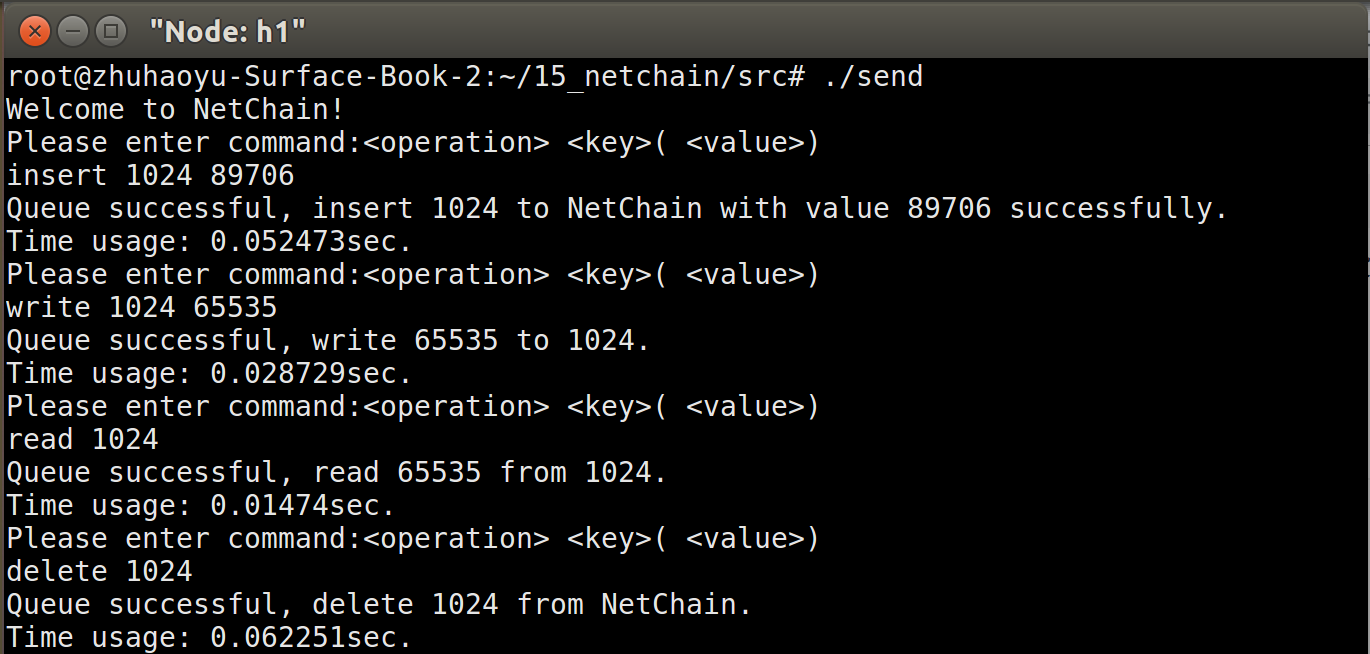
\includegraphics[width=0.8\textwidth]{figures/Evaluation_func_1.png}
    
    \caption{Functionality evaluation: routing, packet parsing, chain generating and queuing}
    \label{fig:Eva_func_1}
\end{figure}



Then we manually down all links between s3 and its neighbors to simulate a switch failure. Now most of the packets will be dropped, only a few packets(doesn't go through s3 or read from other nodes) will have a reply.

\begin{figure}[h]
    \centering
    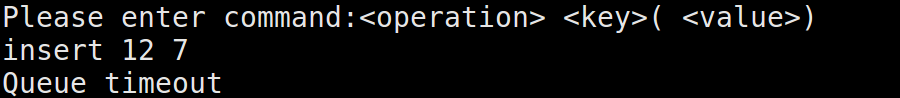
\includegraphics[width=0.8\textwidth]{figures/Evaluation_func_fail.png}
    
    \caption{Functionality evaluation: Queue error when links down}
    \label{fig:Eva_func_fail}
\end{figure}

\begin{figure}[h]
    \centering
    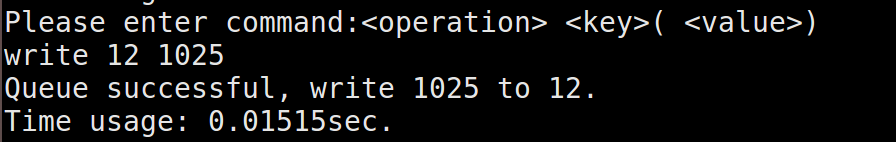
\includegraphics[width=0.8\textwidth]{figures/Evaluation_func_fail2.png}
    
    \caption{Functionality evaluation: Successful queue when fail-over is presented}
    \label{fig:Eva_func_fail}
\end{figure}

At controller, we entered 's3' as the parameter of fail-over, after several milliseconds, the entrys will be added to its neighbors' tables. When it finished, the queue processing will have a reply again.

When fail-over is finished, input anything can start the recovery process. The failed nodes will be randomly assigned to other switches to archive the f node fault-tolrance.

\subsection{Performance}

Here we used 4 different scenarios in evaluation program to test the performance: single host insert performance, single host write performance, single host read performance and single node multi-thread throughput.

\begin{enumerate}
    \item single host insert performance
    
    We inserted 4096 keys to NetChain to test its insert performance. The result is in \texttt{performance/Insert\_4096 keys.log}:
    
   \begin{lstlisting}
Inserting 4096 keys to Netchain finished. Statistics:
Succeed insertings : 4096
Failed insertings  : 0
Success rate       : 1
Time used          : 244.953	sec
Time used per key  : 0.0598031	sec
    \end{lstlisting}

\item single host write performance

    We write values to random keys to NetChain to test its writing performance. The test lasts 30 seconds. The result is in \texttt{performance/Write\_30 sec.log}:
    
   \begin{lstlisting}
writing 3547 keys to Netchain finished. Statistics:
Succeed writings   : 3547
Failed writings    : 0
Success rate       : 1
Time used          : 30.0033sec
Time used per key  : 0.00845877sec
    \end{lstlisting}    


\item single host read performance

    We write values to random keys to NetChain to test its writing performance. The test lasts 30 seconds. The result is in \texttt{performance/Read\_30 sec.log}:
    
   \begin{lstlisting}
Reading 6442 keys to Netchain finished. Statistics:
Succeed readings   : 6442
Failed readings    : 0
Success rate       : 1
Time used          : 30.0043sec
Time used per key  : 0.00465761sec
    \end{lstlisting}    


Here from the previous 3 scenarios, we can figure out that the Insert operation is way slower than write and read. And the write operation needs to travel 3 switchs (in project) to finish the operation while read opeation needs to go through only one. 



\item single node multi-thread throughput

    In this scenario we tested the performance using 1,2,4,8,16 threads, each test lasts 30 seconds. In each test, every thread will randomly generate read or write operations and send it to switch. To better test the real throughput, the timeout of a queue is set to 100ms. If a packet is timeout, it will retry for five times. Which means, a failed queuing means failed for 5 retries. The result is in \texttt{performance/Throughput\_*.log}:
    
   \begin{lstlisting}
1 Thread:
Queueing 4810 keys to Netchain finished. Statistics:
Succeed Queues     : 4810
Failed Queues      : 0
Success rate       : 1
Time used          : 30.0086 sec
Time used per key  : 0.0062388 sec
Throughput   : 160.287Queue/sec

2 Thread:
Queueing 6126 keys to Netchain finished. Statistics:
Succeed Queues     : 6126
Failed Queues      : 0
Success rate       : 1
Time used          : 30.0099 sec
Time used per key  : 0.00489878 sec
Throughput   : 204.132Queue/sec

4 Thread:
Queueing 9521 keys to Netchain finished. Statistics:
Succeed Queues     : 9521
Failed Queues      : 0
Success rate       : 1
Time used          : 30.0167 sec
Time used per key  : 0.00315268 sec
Throughput   : 317.19Queue/sec

8 Thread:
Queueing 12616 keys to Netchain finished. Statistics:
Succeed Queues     : 12617
Failed Queues      : 0
Success rate       : 1.00008
Time used          : 30.0433 sec
Time used per key  : 0.00238137 sec
Throughput   : 419.927Queue/sec

16 Thread:
Queueing 14332 keys to Netchain finished. Statistics:
Succeed Queues     : 14334
Failed Queues      : 0
Success rate       : 1.00014
Time used          : 30.0475 sec
Time used per key  : 0.00209653 sec
Throughput   : 476.979Queue/sec

32 Thread:
Queueing 11744 keys to Netchain finished. Statistics:
Succeed Queues     : 11747
Failed Queues      : 0
Success rate       : 1.00026
Time used          : 30.0882 sec
Time used per key  : 0.00256201 sec
Throughput   : 390.319Queue/sec

    \end{lstlisting}

Here we can found that if we increase the threads, the queue throughput increases dramatically. But due to the cost of switching threads, The highest throughput occurs when using around , which is around 400 Queue per second.

\end{enumerate}


\subsection{Robust}
Here we tested the system stability when failure occurs. We uses 2 scenarios to show the system stability when fast fail-over and recovery is performed.
\begin{enumerate}



\item fast fail-over performance

In this scenario, we start 2 xterm terminals. Host h1 will do write operation for 30 seconds and h2 will do read operations. When they are functioning, the link between s3 and its neighbor will be manually down, and after approximately 5 seconds, the fail-over will perform. We will calculate the time used between fast fail-over is applied and network is back to work again. The result is in \texttt{Failover\_read.log} and \texttt{Failover\_write.log}.

\begin{lstlisting}
Reading 4367 keys to Netchain finished. Statistics:
Succeed readings   : 4349
Failed readings    : 18
Success rate       : 0.995878
Time used          : 30.0037sec
Time used per key  : 0.00687055sec

writing 2574 keys to Netchain finished. Statistics:
Succeed writings   : 2556
Failed writings    : 18
Success rate       : 0.993007
Time used          : 30.0032sec
Time used per key  : 0.0116562sec
    \end{lstlisting}

In fact, when links are manually down, the system drops most packets since they need to go through this switch. But when fast-failover is performed, it back to work in less than 1 queue timeout. I.e. when we start to do fast-failover, 


\item recovery time performance

In this scenario, we start 2 xterm terminals after fail-over is done. Host h1 will do write operation for 30 seconds and h2 will do read operations. When they are functioning, the fail recovery script is activated, and the write queue will be put on hold several times. We will calculate the queue successful rate when the recovery is in progress. The result is in \texttt{Recovery\_read.log} and \texttt{Recovery\_write.log}.


\begin{figure}[htbp]
    \centering
    \begin{minipage}[t]{0.48\textwidth}
    \centering
    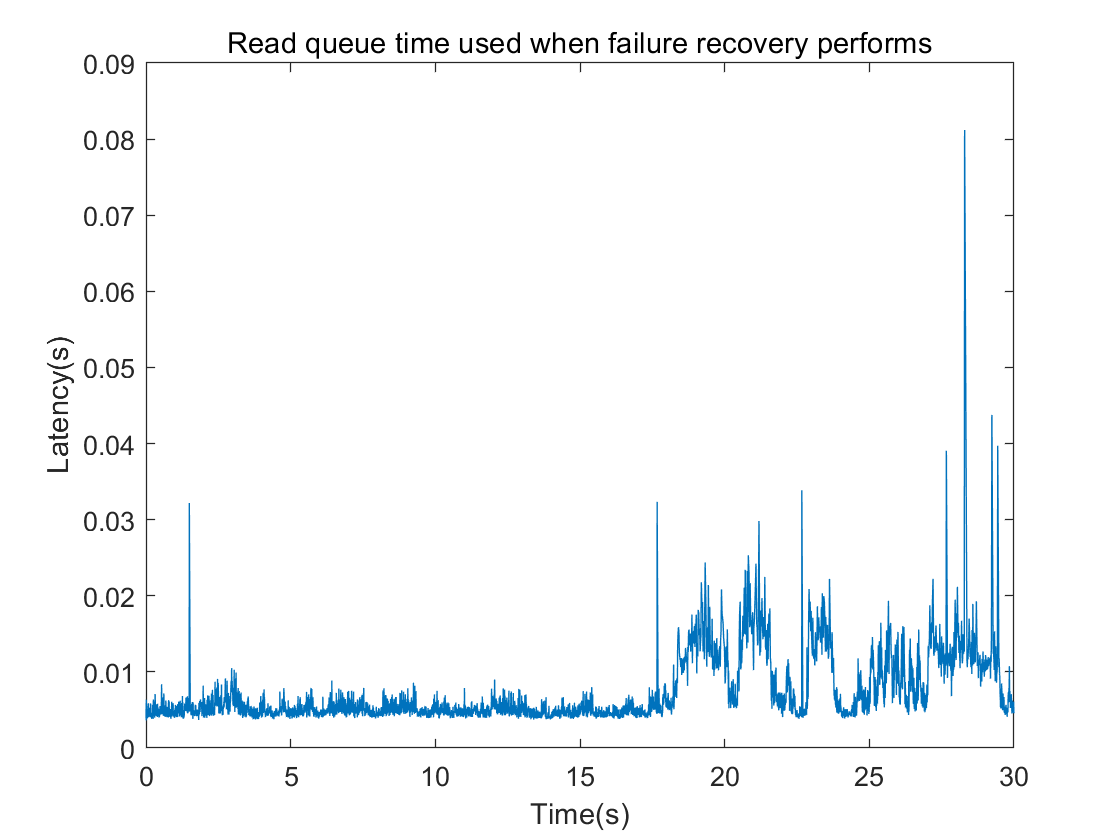
\includegraphics[width=0.6\textwidth]{figures/Recovery_read_latency.png}
    \caption{Read latency when recovery performs}
    \label{fig:my_label}
    \end{minipage}
    \begin{minipage}[t]{0.48\textwidth}
    \centering
    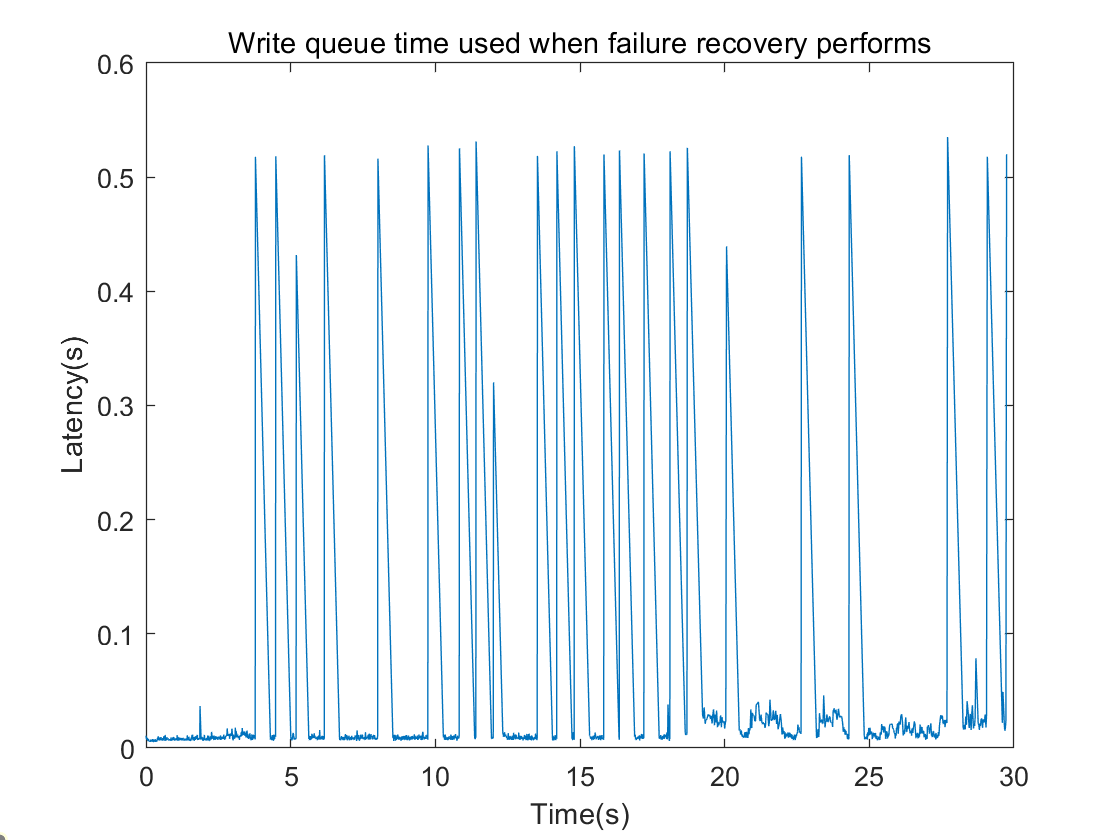
\includegraphics[width=0.6\textwidth]{figures/Recovery_write_latency.png}
    \caption{Write latency when recovery performs}
    \label{fig:my_label}
    \end{minipage}
    
\end{figure}

\begin{figure}
    \centering
    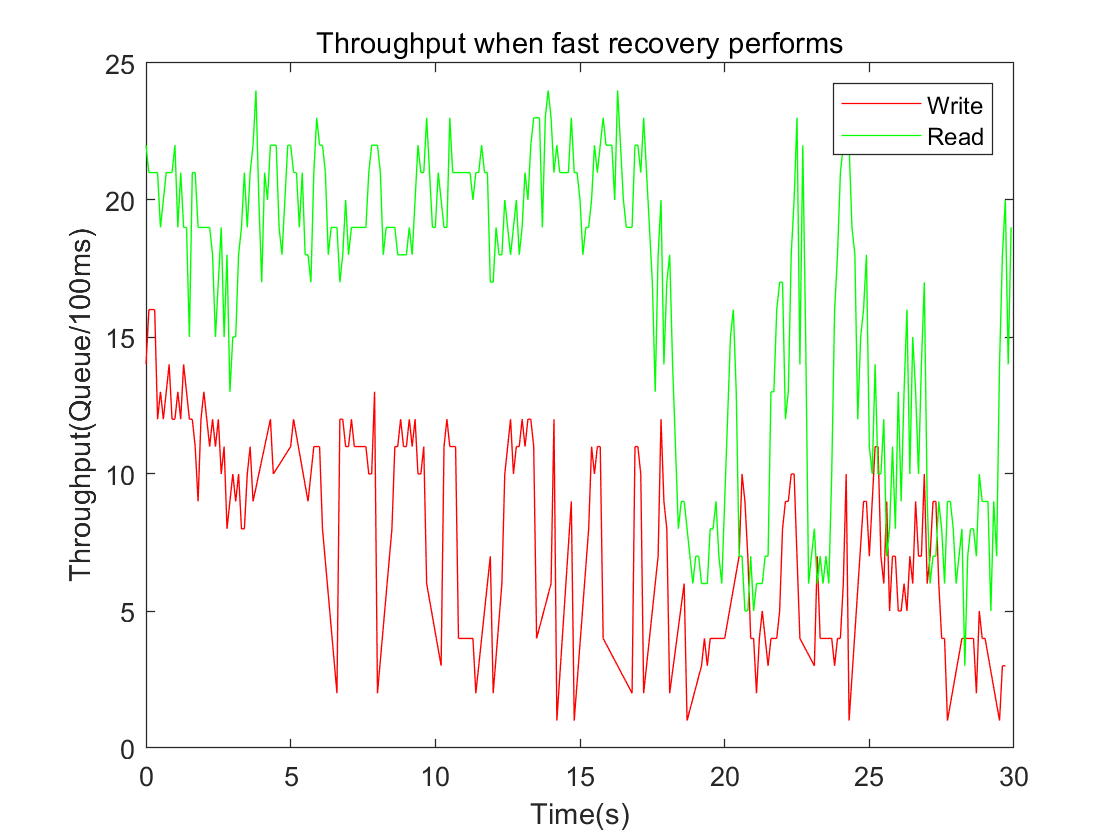
\includegraphics[width=0.6\textwidth]{figures/Recovery_thrp.png}
    \caption{Throughput when recovery performs}
    \label{fig:my_label}
\end{figure}
\begin{lstlisting}
Reading 4902 keys to Netchain finished. Statistics:
Succeed readings   : 4902
Failed readings    : 0
Success rate       : 1
Time used          : 30.0028sec
Time used per key  : 0.00612051sec

writing 1689 keys to Netchain finished. Statistics:
Succeed writings   : 1669
Failed writings    : 20
Success rate       : 0.988159
Time used          : 30.2643sec
Time used per key  : 0.0179185sec
    \end{lstlisting}
    
In this evaluation we can see that when doing recovery, only few writing packets are dropped even 4096 keys is stored in NetChain, and reading packets is never influenced.




\end{enumerate}

\section{Conclusion}
\subsection{Work summary}
In our project, we reproduced the paper "NetChain: Scale-Free Sub-RTT Coordination" in a p4 way. The project successfully implemented and tested most functionalities concerned in the paper. In a coordination between p4 switch and a python-based controller script, our project can perform basic functionalities:  node assignment, key-value storage and chain routing. Also the reproduced project can handle a fail-over and recovery when switch failure occurs. The project is based on Software Defined Networks(SDN) and over normal routing algorithms. It shows the probability and feasibility of offloading the key-value storage to switch data-plane to boost the IO speed when doing key-value storage. The project also shows that this well-designed chain replication have a strong fault-tolerance which can handle f error nodes when f+1 nodes are contained in a chain. 

\subsection{Future works and expectations}

In this project, most the functionality is implemented and works perfectly, but what is expected but missing is the scalability of the chain. In our project, we have a way and framework to scale the chain, but do not have enough time to finish it. Moreover, in the paper, the authors talked about the value size scalability. when a value is too large for one packet to carry or for switch on-chip register to store, there is one possible way is to divide it into several parts and store it in several key-value pairs. 

In the implementation of the project we also founds some disadvantages in the paper that may need to be solved. First is about the matching table size usage. Apparently every key needs more than two entries. One is for reading and another one is for writing. When fail recovery performs, the recovery table of the neighbor switch of the failed one will be filled with all keys and destinations to the newly assigned switch. Another is the fail recovery sync problems. In the paper it said that they will monitor the registers between source switch and destination switch. In our project we designed a new packet operation called "transfer", which is not implemented due to the time. It reads value from the source switch and write it to destination switch, which is performed with sequence number to keep consistency.


\label{lastpage} % this must stay here
\clearpage
\addcontentsline{toc}{section}{References}
\bibliographystyle{acm}
\bibliography{refs}

\clearpage
\appendix
\pagenumbering{Roman}

\section{Group organization}


\paragraph{Haoyu Zhu}

\begin{enumerate}
     \item Netchain Header defined, Parser of NetChain finished, Write and Read Queue.
    \item Forwarding and routing.
    \item Implement sequence on switch but not host to enable parallal operations.
    \item Fast-recovery dealing.
    \item Topology init and routing table filling.
    \item Generate and send Netchain queues.
    \item Scapy Netchain header defined
    \item NetChain node routing.
    \item Evaluation script and program.
    \item Report of implementation of hosts.
\end{enumerate}
 


\paragraph{Francisco Dumont}
\begin{enumerate}
    \item Forwarding and routing.
    \item NetChain runtime table filling.
    \item Filling index table and implement Insert and Delete function. Francisco.
    \item Fast-failover table filling. Francisco.
    \item Fast recovery when failure occurs.
    \item Generate and send Netchain queues.
    \item Most part of report, including Introduction, Abstract, Paper review, Implementation of controller and switch.
\end{enumerate}

Francisco have a lot of contributions to the implementation part, Althouth some code may not be used at last, He meets every week with Haoyu at satursday, and works when he is free. Haoyu have developed Host program, more than half of the switch code and at last week, he changed some codes in controller because of our misunderstanding of paper.


\end{document}